\part{Analyse des données textuelles}

    \chapter{Caractéristiques générales du jeu de données}

        Dans toute cette analyse, on se basera sur les données manuellement étiquetées (ou ground truth), échantillon de 500 fiches techniques avec les listes d'ingrédients associées.
        Le code ayant servi à effectuer ces analyses est présenté dans le notebook en annexe \mref{code:text_analysis}.

        \section{Volumétrie}

        TODO peut-etre : Produits par type, avec les comptes, du PIM et de la GT, avec l'axe en qualité et hors qualité.

        TODO peut-etre : Textes renseignés vs. pas renseignés.



        \section{Distributions des longueurs des textes}

        TODO peyut-être : Longueur des listes d'ingrédients dans le PIM, fonction du type de produit.

        L'analyse des longueurs des textes montre que les listes d'ingrédients sont en moyenne longues de 400 caractères, et le contenu des documents de 4000 caractères (cf. \reftable{tbl:text_lengths}).
        La distribution des longueurs de listes d'ingrédients et des longueurs de textes est présentée à la \reffig{fig:text_length}, et leur représentation de l'une en fonction de l'autre à la \reffig{fig:text_length_2}.
        Il apparaît qu'il n'y a pas de corrélation entre la longueur de la liste d'ingrédients et la longueur du contenu du document ($r^{2} = 0.139$).
        \begin{table}[htbp]
            \begin{center}
            {\scriptsize
            \begin{tabular}{lcccccccc}
\toprule
{} & \multicolumn{8}{l}{text} \\
{} &  count &      mean &          std &  min &      25\% &     50\% &      75\% &      max \\
\midrule
\textbf{Texte des documents } &  500.0 &  3937.630 &  3280.860732 &  0.0 &  2173.75 &  3247.5 &  5034.25 &  37322.0 \\
\textbf{Listes d'ingrédients} &  500.0 &   199.686 &   457.044723 &  0.0 &    43.00 &   122.0 &   250.75 &   7963.0 \\
\bottomrule
\end{tabular}

            }
            \caption{Longueur des textes dans le dataset}
            \label{tbl:text_lengths}
            \end{center}
        \end{table}       
        \begin{figure}[htbp]
            \begin{center}
            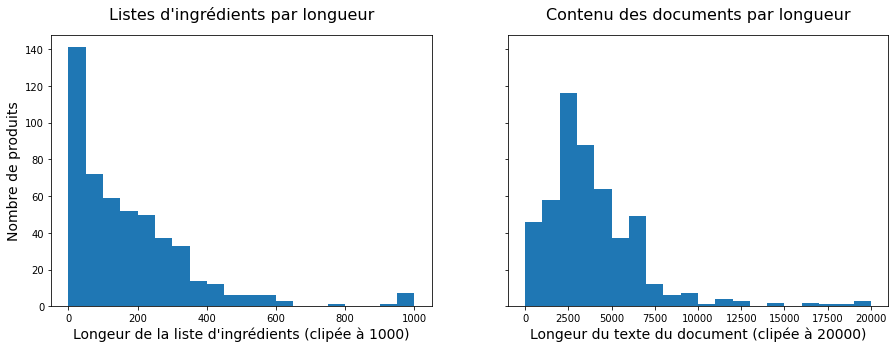
\includegraphics[width=0.9\linewidth]{img/text_lengths.png}
            \end{center}
            \caption{Distribution des longueurs de textes}
            \label{fig:text_length}
        \end{figure}     
        \begin{figure}[htbp]
            \begin{center}
            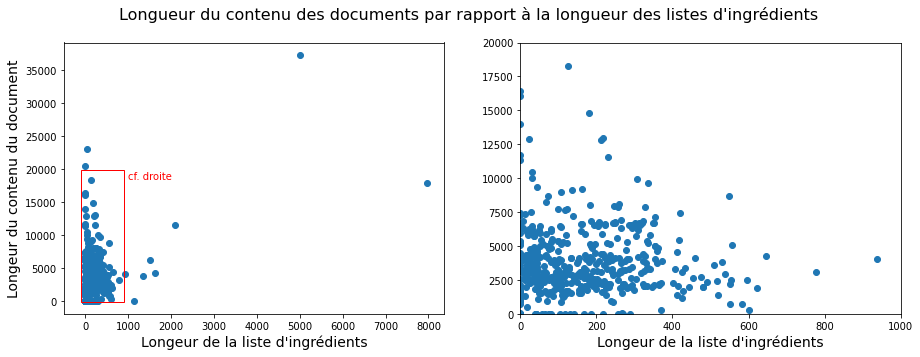
\includegraphics[width=0.9\linewidth]{img/text_lengths_2.png}
            \end{center}
            \caption{Corrélation entre longueurs des textes}
            \label{fig:text_length_2}
        \end{figure}     
        
        
    \chapter{Analyse textuelle}

        \section{Mots de chacun des corpus}

        Pour l'analyse des mots de chacun des corpus (listes d'ingrédients et contenu des documents), on fait d'abord un preprocessing de ces textes bruts :
        \begin{itemize}
            \item mise en minuscule de ces textes
            \item retrait des accents
            \item retrait des stopwords suivants : {'pas', 'le', 'en', 'pour', 'ou', 'ce', 'de', 'dans', 'du', 'and', 'un', 'sur', 'et', 'of', 'est', 'par', 'la', 'les', 'dont', 'au', 'des', 'que'}
            \item split des textes à chaque whitespace (espace, tabulation, retour à la ligne, \dots)
        \end{itemize}
        La liste de ces stopwords a été manuellement établie à partir des mots les plus fréquents de chacun des vocabulaires.
        Elle est commune aux deux corpus.
        Un descriptif des vocabulaires est présenté à la \reftable{tbl:vocabularies}.
        Un rapide parcours de ces exemples montre que l'utilisation des mots dans ces deux corpus (ingrédients et contenu des documents) est différente.
        On s'attend à pouvoir différencier automatiquement ces types de textes.
        Le vocabulaire des ingrédients est, comme on pouvait s'y attendre, entièrement inclus dans le vocabulaire du contenu des fiches techniques.
        
        {\renewcommand{\arraystretch}{1.5}%
        \begin{table}[htbp]
            \begin{center}
            {\scriptsize
            \begin{tabular}{lcc}
    \toprule
    {} &  \textbf{Ingrédients} &  \textbf{Contenu des documents} \\
    \midrule
    \textbf{Longueur du vocabulaire      } &  1324 & 15465 \\
    \hline
    \multirow{20}*{\textbf{Top 20 mots}} &sucre       : 363 occurences & produit     : 2198 occurences \\
    &acide       : 255 occurences & non         : 2164 occurences \\
    &sel         : 240 occurences & produits    : 1508 occurences \\
    &sirop       : 180 occurences & 10          : 1404 occurences \\
    &eau         : 178 occurences & kg          : 1290 occurences \\
    &poudre      : 176 occurences & base        : 1119 occurences \\
    &arome       : 175 occurences & sel         : 1041 occurences \\
    &lait        : 171 occurences & poids       : 1021 occurences \\
    &ble         : 171 occurences & 100         : 971 occurences \\
    &huile       : 146 occurences & palette     : 933 occurences \\
    &citrique    : 132 occurences & ingredients : 917 occurences \\
    &farine      : 128 occurences & date        : 904 occurences \\
    &amidon      : 125 occurences & sucre       : 841 occurences \\
    &glucose     : 124 occurences & 12          : 803 occurences \\
    &cacao       : 122 occurences & code        : 801 occurences \\
    &extrait     : 117 occurences & lait        : 733 occurences \\
    &acidifiant  : 114 occurences & absence     : 697 occurences \\
    &aromes      : 98 occurences & fiche       : 688 occurences \\
    &soja        : 96 occurences & the         : 658 occurences \\
    &concentre   : 92 occurences & france      : 657 occurences \\
    \bottomrule
\end{tabular}
            }
            \caption{Caractéristiques des vocabulaires}
            \label{tbl:vocabularies}
            \end{center}
        \end{table}
        }

        \section{Répartitions des mots dans et hors des listes d'ingrédients}

        On calcule la \og document frequency \fg des mots du corpus des ingrédients dans les listes d'ingrédients.
        Elle s'étend simplement au corpus du contenu des documents en la mettant à 0 pour les mots qui n'appartiennent pas au vocabulaire des ingrédients.
        Cela permet de calculer un score absolu $s_{i}$ pour chaque mot $i$ via la formule suivante :
        \[s_{i} = \log_{2}(1 + c_{i})\]
        où $c_{i}$ est le nombre de listes d'ingrédients dans lequel le mot $i$ apparaît (proportionnel à la document frequency).
       
        Le score absolu vaut donc $0$ si le mot n'est pas présent dans le vocabulaire des ingrédients, $1$ s'il est présent une fois, et progresse de manière logarithmique en fonction du taux de présence du mots dans le corpus des ingrédients (c'est une \og smooth document frequency \fg).
        On peut, de manière similaire, calculer un score pour l'ensemble des mots, relatif à la présence dans le contenu des documents.
        Attention, dans la mesure où la composition est normalement portée par la fiche technique, en théorie les mots de la liste d'ingrédients sont contenus dans le texte du document.
        Pour prendre en compte ce point, avant de calculer le score par rapport au contenu des documents, on soustrait les comptes des mots de la liste d'ingrédients des comptes de mots du contenu du document.
        Ne sont considérés comme apparaissant dans le contenu du document que les mots dont la différence est strictement positive.
        Une illustration de ces scores est donnée à la \reffig{fig:scores_bar}.

        \begin{figure}[htbp]
            \begin{center}
            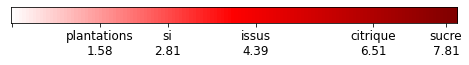
\includegraphics[width=0.6\linewidth]{img/scores_bar.png}
            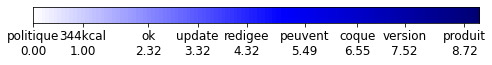
\includegraphics[width=0.6\linewidth]{img/corpus_score_bar.png}
            \end{center}
            \caption{Exemples de scores absolus de mots}
            \label{fig:scores_bar}
        \end{figure}

        La \reftable{tbl:vocabularies} montre que certains mots sont répandus à la fois au sein des listes d'ingrédients, mais également dans le corps des documents (ex: \og sel \fg, \og sucre \fg, \og lait \fg, \dots).
        L'identification des listes d'ingrédients devrait être plus efficace si on prend en compte la fréquence relative des mots dans chacun des corpus : 
        \begin{itemize}
            \item la présence du mot \og sucre \fg, bien qu'il soit très souvent présent dans les listes d'ingrédients, n'est pas forcément un bon indicateur que le bloc de texte considéré est une liste d'ingrédients
            \item le mot \og poids \fg devrait pénaliser fortement un bloc de texte car il n'est pas présent dans les listes d'ingrédients, mais fréquemment à l'extérieur
        \end{itemize}
        On peut calculer un score relatif $s'_{i}$ pour chaque mot $i$ via la formule suivante :
        \[s'_{i} = \log_{2}(\frac{1 + c^{ingred}_{i}}{1 + c^{docs}_{i}}) = log_{2}(1 + c^{ingred}_{i}) - log_{2}(1 + c^{docs}_{i}) = s^{ingred}_{i} - s^{docs}_{i}\]
        où $c^{corpus}_{i}$ est le nombre de documents du corpus $corpus$ dans lequel le mot $i$ apparaît, et $s^{corpus}_{i}$ est le score absolu du mot $i$ dans le corpus $corpus$ tel que défini précédemment.
        Cette manière de calculer le score : 
        \begin{itemize}
            \item fait qu'un mot autant présent (au sens de la document frequency) dans les deux corpus a un score de $0$
            \item un mot 2 fois plus présent dans le corpus des ingrédients que dans le corpus des documents aura un score de $1$
            \item un mot plus présent dans le corpus des documents que dans le corpus des ingrédients aura un score négatif
            \item un mot plus présent dans le corpus des ingrédients que dans le corpus des documents aura un score positif
            \item peut fonctionner parce que la taille des corpus est équilibrée (il faudrait passer en document frequency en cas de déséquilibre)
        \end{itemize}
        Une illustration de ces scores est présentée à la \reffig{fig:relative_score_bar}.

        \begin{figure}[htbp]
            \begin{center}
            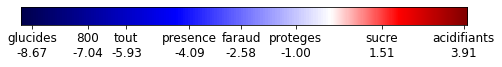
\includegraphics[width=0.6\linewidth]{img/relative_score_bar.png}
            \end{center}
            \caption{Exemples de scores relatifs de mots}
            \label{fig:relative_score_bar}
        \end{figure} 


        \section{Représentations graphiques des textes et mots}

            \subsection{Vectorisation des mots}

            On calcule les embeddings des mots via l'algorithme Word2Vec, sur le corpus du contenu des documents.
            Si l'on applique deux méthode de réduction de la dimensionnalité sur ces embeddings (PCA et ISOMAP), on peut en faire une représentation graphique.
            Le résultat de cette projection est présenté à la \reffig{fig:word2vec_projection}.
            On voit clairement que les embeddings des mots issus du vocabulaire des ingrédients sont localisés dans les mêmes régions.
            Le calcul des embeddings via l'algorithme Word2Vec semble donc avoir un intérêt pour l'identification des listes d'ingrédients. 

            \begin{figure}[htbp]
                \begin{center}
                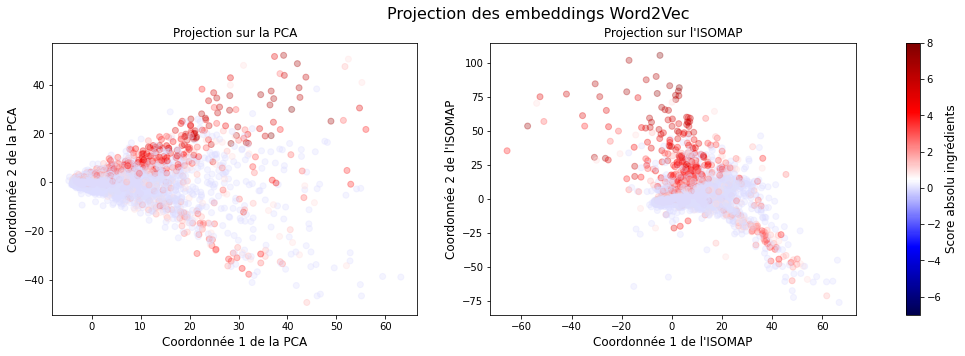
\includegraphics[width=0.9\linewidth]{img/word2vec_projection.png}
                Remarque : ci-dessus, la colormap a très légèrement été décalée pour que les mots ayant un score de 0 soient visibles (gris/bleu clair) - scores absolus
                \bigskip
                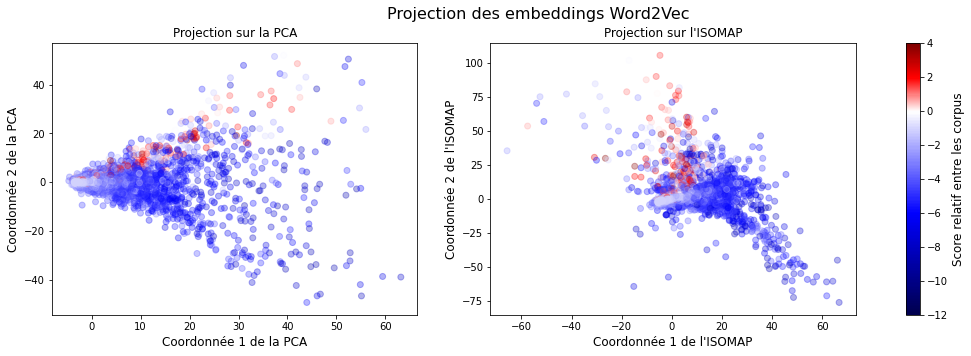
\includegraphics[width=0.9\linewidth]{img/word2vec_projection_relative.png}
                \end{center}
                \caption{Projection des embeddings Word2Vec}
                \label{fig:word2vec_projection}
            \end{figure}            

            \subsection{Vectorisation des textes}

            La vectorisation des textes va se faire sur la base de la matrice des comptes ou des fréquences de mots.
            On commence par effectuer une PCA (après standardisation) sur les comptes de mots de chacun des textes : listes d'ingrédients ou contenu des documents.
            Les résultats sont présentés à la \reffig{fig:PCA_counts}.            
            \begin{figure}[htbp]
                \begin{center}
                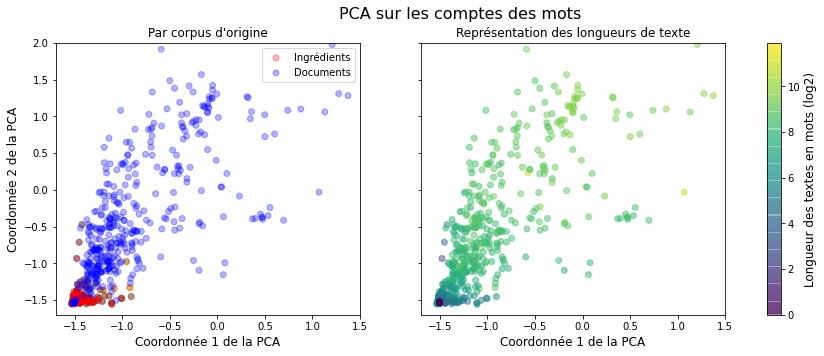
\includegraphics[width=0.9\linewidth]{img/PCA_counts.png}
                \end{center}
                \caption{Projection des comptes : PCA}
                \label{fig:PCA_counts}
            \end{figure}
            Les corpus sont bien séparés. 
            Une explication pour cette séparation assez franche est la suivante : les vecteurs du corpus des contenus de documents ont en général une norme plus élevée que celle des ingrédients.
            La dispersion est donc plus grande pour les contenus des documents que pour les ingrédients.            

            On peut appliquer une transformation similaire, mais cette fois en utilisant une Truncated SVD (cf. \reffig{fig:tSVD_counts}).
            \begin{figure}[htbp]
                \begin{center}
                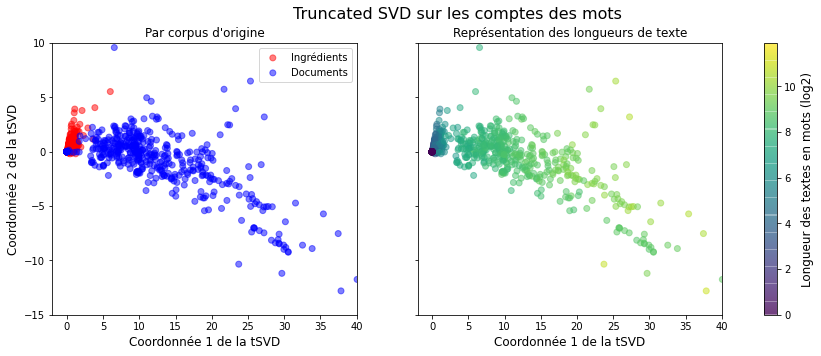
\includegraphics[width=0.9\linewidth]{img/tSVD_counts.png}
                \end{center}
                \caption{Projection des comptes : Truncated SVD}
                \label{fig:tSVD_counts}
            \end{figure}
            Là encore, les deux corpus sont différemment localisés.
            La même explication que pour les résultats de la PCA pourrait tenir pour expliquer cette répartition différenciée.

            On peut changer d'espace de départ, en se basant sur les fréquences (\og term-frequencies \fg) d'apparition des mots dans les textes. 
            Cela permet de countourner le problème des longueurs différentes des textes.
            L'application d'une PCA est présentée à la \reffig{fig:PCA_freq}.
            \begin{figure}[htbp]
                \begin{center}
                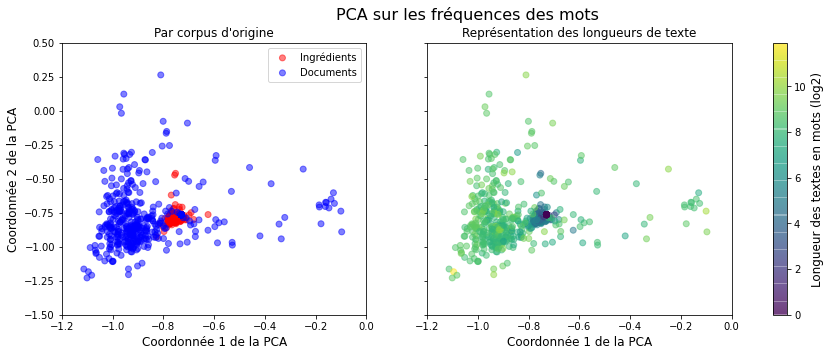
\includegraphics[width=0.9\linewidth]{img/PCA_freq.png}
                \end{center}
                \caption{Projection des fréquences : PCA}
                \label{fig:PCA_freq}
            \end{figure}
            Les textes correspondant aux ingrédients sont à nouveau localisés dans la même région, bien que cette fois les normes des vecteurs de l'espace de départ soient comparables entre les deux corpus.
            Une explication serait que les nombreux \og trous \fg dans les vecteurs correspondants aux ingrédients (pour rappel, le vocabulaire des ingrédients est plus de 10 fois plus petit que le vocabulaire des documents, cf. \reftable{tbl:vocabularies}) les cantonnent à un partie limité de l'espace de départ.
            D'où la similarité dans l'espace de la PCA.


            Enfin, si on applique une Truncated SVD sur les fréquences de mots, on observe à nouveau une séparation franche des corpus.
            Le résultat est présenté à la \reffig{fig:tSVD_freq}.
            \begin{figure}[htbp]
                \begin{center}
                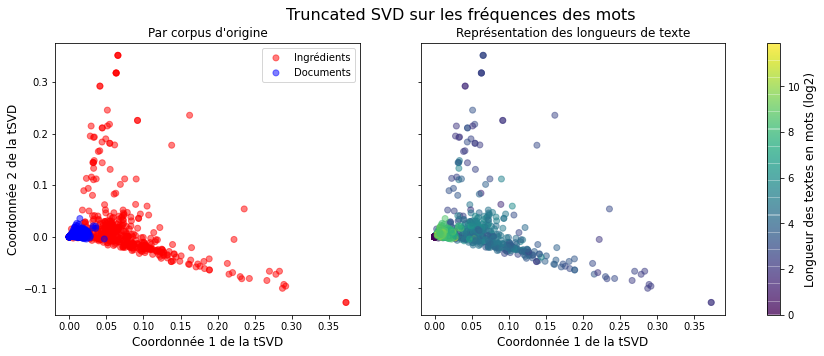
\includegraphics[width=0.9\linewidth]{img/tSVD_freq.png}
                \end{center}
                \caption{Projection des fréquences : Truncated SVD}
                \label{fig:tSVD_freq}
            \end{figure}
            Cette fois, c'est le corpus des documents qui occupe une région limitée de la représentation.
            On peut expliquer ce point par le fait que du fait que les listes d'ingrédients sont courtes, les \og term frequencies \fg sont élevées (le diviseur étant relativement plus petit).
            Les vecteurs des listes d'ingrédients contribuent donc à des valeurs singulières importantes, et leurs projections dans les espaces correspondant sont plus longues.
            
            On observe de plus deux \og moustaches \fg distinctes (proches des axes de cette projection, cf. \reffig{fig:tSVD_freq_groups}).
            \begin{figure}[htbp]
                \begin{center}
                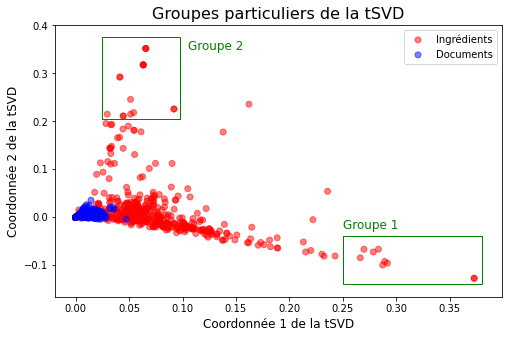
\includegraphics[width=0.9\linewidth]{img/tSVD_freq_groups.png}
                \end{center}
                \caption{Groupes particuliers dans la tSVD des fréquences}
                \label{fig:tSVD_freq_groups}
            \end{figure}    
            Si on compare les textes de ces deux groupes de points, on s'aperçoit que des tendances nettes se dégagent (cf. \reftable{tbl:tSVD_sample}):
            \begin{itemize}
                \item comme anticipé, il s'agit de listes d'ingrédients relativement courtes (d'où leur norme importante dans cet espace)
                \item la moustache de droite reprend des listes d'ingrédients correspondant principalement à du thon ou des mono-légumes en boite (des conserves)
                \item la moustache du haut correspond essentiellement à des pâtes ou des mono-produits d'épicerie (épices, farine, thé, café)        
            \end{itemize}           
            {\renewcommand{\arraystretch}{1.5}%
            \begin{table}[htbp]
                \begin{center}
                {\scriptsize
                \begin{tabular}{lp{9cm}cc}
\toprule
{} &                                                                Texte &         x &         y \\
\midrule
Groupe 1 &                                                       Thon, eau, sel &  0.373079 & -0.127052 \\
Groupe 1 &                                              Pois chiches, eau, sel. &  0.266423 & -0.084501 \\
Groupe 1 &                                            Haricots beurre, eau, sel &  0.283409 & -0.066561 \\
Groupe 1 &                                           Câpres, eau, vinaigre, sel &  0.291819 & -0.095479 \\
Groupe 1 &                                              Thon albacore, eau, sel &  0.287423 & -0.099627 \\
Groupe 1 &                                            Eau, haricots verts, sel. &  0.278588 & -0.072474 \\
Groupe 1 &                                           Pommes de terre, eau, sel. &  0.289291 & -0.092162 \\
Groupe 1 &                                  Carottes rondelles, eau, sel, sucre &  0.269849 & -0.066600 \\
Groupe 1 &                                                       Thon, eau, sel &  0.373079 & -0.127052 \\
\midrule    
Groupe 2 &                      - 100\% Semoule de blé dur de qualité supérieure &  0.065551 &  0.351800 \\
Groupe 2 &                                                 100\% haricots blancs &  0.051373 &  0.214921 \\
Groupe 2 &                        100\% Semoule de blé dur de qualité supérieure &  0.065551 &  0.351800 \\
Groupe 2 &               Semoule de blé dur* \newline *issu de l'agriculture biologique &  0.054211 &  0.218192 \\
Groupe 2 &                                                      Tilleul (100\%). &  0.041323 &  0.292199 \\
Groupe 2 &                        100\% semoule de blé dur de qualité supérieure &  0.065551 &  0.351800 \\
Groupe 2 &                                                    Farine de blé T45 &  0.092002 &  0.225689 \\
Groupe 2 &        - Semoule de blé dur de qualité supérieure \newline - 30\% oeufs frais &  0.044446 &  0.211188 \\
Groupe 2 &  - 100\% Semoule de blé dur de qualité courante \newline - Contient du gluten &  0.051337 &  0.245649 \\
Groupe 2 &                            SEMOULE DE BLE' DUR de qualité supérieure &  0.063201 &  0.317653 \\
Groupe 2 &                                                         100\% Arabica &  0.041324 &  0.292222 \\
Groupe 2 &                                                       agar-agar 100\% &  0.029466 &  0.214845 \\
Groupe 2 &                            SEMOULE DE BLE' DUR de qualité supérieure &  0.063201 &  0.317653 \\
Groupe 2 &                            SEMOULE DE BLE' DUR de qualité supérieure &  0.063201 &  0.317653 \\
Groupe 2 &                            SEMOULE DE BLE' DUR de qualité supérieure &  0.063201 &  0.317653 \\
Groupe 2 &        - Semoule de blé dur de qualité supérieure \newline - 30\% oeufs frais &  0.044446 &  0.211188 \\
Groupe 2 &                                                    Farine de blé T45 &  0.092002 &  0.225689 \\
\bottomrule
\end{tabular}

                }
                \caption{Longueur des textes dans le dataset}
                \label{tbl:tSVD_sample}
                \end{center}
            \end{table}
            }

            